\documentclass{beamer}
\usepackage{color,amsmath}
\usepackage{subfigure}
\usepackage{booktabs}
\usepackage{framed}
\usepackage{comment}

\usepackage{hyperref}
\hypersetup{
    colorlinks=true,
    linkcolor=blue,
    filecolor=magenta,      
    urlcolor=cyan,
}
 
\def\vf{\vfill}

%%%%%%%%%%%%%%%%%%%%%%%%%%
\title[]{Four areas of difficulty:\\Informed consent, informational risk, privacy, and making decisions in the face of uncertainty}
\author[]{Matthew J. Salganik\\Department of Sociology\\Princeton University}
\date[]{Summer Institute in Computational Social Science\\June 19, 2019
\vfill
\begin{flushleft}
{\scriptsize
The Summer Institutes in Computational Social Science is supported by grants from the Russell Sage Foundation and the Alfred P. Sloan Foundation.}
\end{flushleft}
\begin{flushright}

\includegraphics[width=0.1\textwidth]{figures/cc-by.png}
\end{flushright}
}
\begin{document}
%%%%%%%%%%%%%%%%%%%%%%%%%%
\frame{\titlepage}
%%%%%%%%%%%%%%%%%%%%%%%%%%
\begin{frame}

Applying principles can be hard.  Four area of difficulty:
\begin{enumerate}
\item Informed consent
\item Informational risk
\item Privacy
\item Making decisions in the face of uncertainty
\end{enumerate}

\pause
\vf
Simple idea, Counter-example(s), better idea, advice

\end{frame}
%%%%%%%%%%%%%%%%%%%%%%%%%%%
\begin{frame}

\begin{center}
\Large{Informed consent}
\end{center}

\end{frame}
%%%%%%%%%%%%%%%%%%%%%%%%%%%
\begin{frame}

Simple idea: informed consent from all participants

\end{frame}
%%%%%%%%%%%%%%%%%%%%%%%%%%%
\begin{frame}

\begin{center}

\includegraphics[width=0.9\textwidth]{figures/pager_mark_2003_title.png}\\
\tiny{\url{http://www.jstor.org/stable/10.1086/374403}}
\end{center}
\pause
\vf
Field experiments to study discrimination, at least 117 studies in 17 countries (Riach and Rich, 2002; Rich 2014)\\

\end{frame}
%%%%%%%%%%%%%%%%%%%%%%%%%%%%
\begin{frame}

Principles-based argument
\begin{itemize}
\item the limited harm to the employers
\pause
\item the great social benefit of having reliable measure of discrimination
\pause
\item the weakness of other methods of measuring discrimination
\pause
\item the fact that deception does not strongly violate the norms of that setting
\end{itemize}

\end{frame}
%%%%%%%%%%%%%%%%%%%%%%%%%%%%
\begin{frame}

Rules-based argument
\begin{itemize}
\item Dozens of IRBs approved (probably based on Common Rule §46.116, part (d))
\pause
\item US courts have also supported the lack of consent and use of deception in field experiments to measure discrimination (No. 81-3029.
US Court of Appeals, 7th Circuit).
\end{itemize}

\end{frame}
%%%%%%%%%%%%%%%%%%%%%%%%%%%%
\begin{frame}

\begin{itemize}
\item Simple idea: informed consent for all research
\pause
\item Actual rules and principles: some for of consent for most research
\end{itemize}

\end{frame}
%%%%%%%%%%%%%%%%%%%%%%%%%%%%
\begin{frame}

\begin{itemize}
\item Is desire for consent motivated by respect for persons or beneficence? (think Encore)
\pause
\item Ideas for alternatives in \href{https://www.bitbybitbook.com/en/1st-ed/preface/}{Bit by Bit, Sec 6.6.1}
\end{itemize}

\end{frame}
%%%%%%%%%%%%%%%%%%%%%%%%%%%%
\begin{frame}

\begin{center}
\Large{Understanding and managing informational risk}
\end{center}

\end{frame}
%%%%%%%%%%%%%%%%%%%%%%%%%%%
\begin{frame}

Biggest risk from much of computational social science is informational risk.  Harms from the disclosure of personal information could be: 

\begin{itemize}
\item economic (e.g., losing a job)
\item social (e.g., embarrassment)
\item psychological (e.g., depression)
\item criminal (e.g., arrest for illegal behavior)
\end{itemize}

\end{frame}
%%%%%%%%%%%%%%%%%%%%%%%%%%%
\begin{frame}

Simple idea: Data can be made anonymous, and we can tell what data is sensitive

\end{frame}
%%%%%%%%%%%%%%%%%%%%%%%%%%%
\begin{frame}

\begin{center}
\only<1>{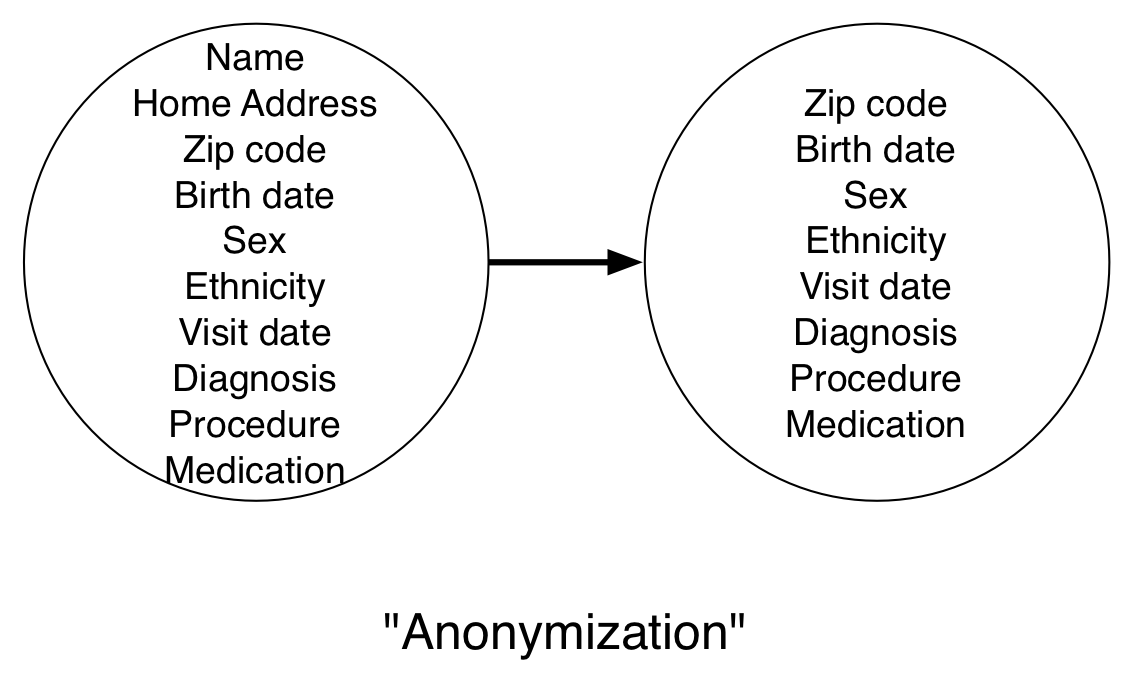
\includegraphics[width=0.9\textwidth]{figures/anonymization.png}}
\only<2>{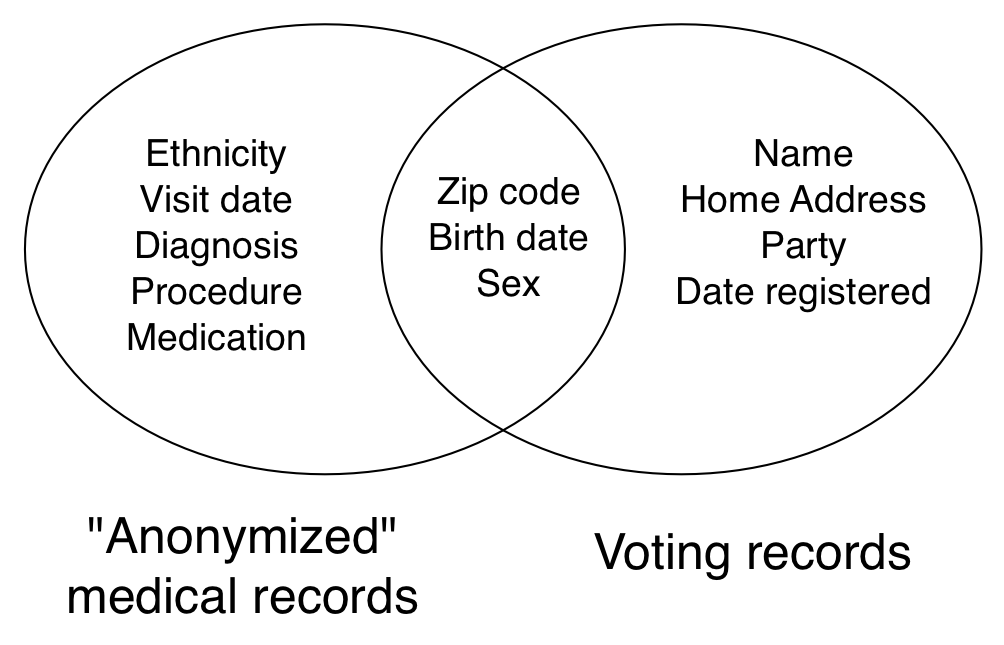
\includegraphics[width=0.9\textwidth]{figures/re-identified.png}}
\end{center}

\vf
\href{http://dx.doi.org/10.1142/S0218488502001648}{Sweeney (2002)}

\end{frame}
%%%%%%%%%%%%%%%%%%%%%%%%%%%
\begin{frame}

Risks come from combining data sources\\
\vf
\begin{minipage}[c]{0.35\textwidth}
$\underbrace{\text{Baking soda}}_{\text{Safe}} + \underbrace{\text{Vinegar}}_{\text{Safe}} =$
\end{minipage}
\hspace{0.05\textwidth}
\begin{minipage}[c]{0.55\textwidth}
\onslide<2>{
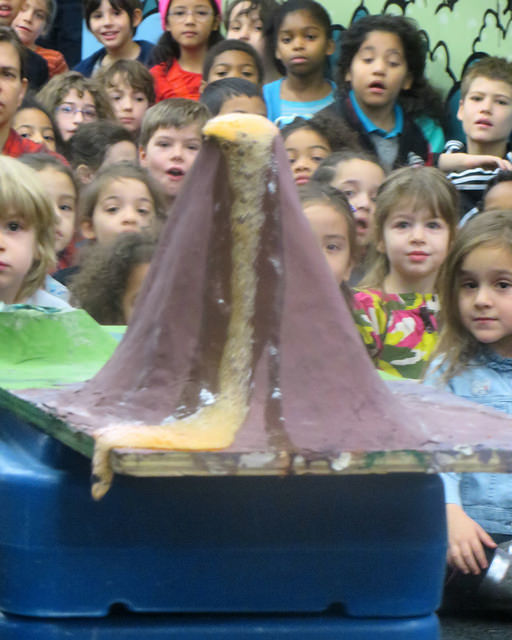
\includegraphics[width=0.8\textwidth]{figures/baking_soda_volcano}\\ {\tiny \url{https://www.flickr.com/photos/edenpictures/15962352215/}}
}
\end{minipage}

\end{frame}
%%%%%%%%%%%%%%%%%%%%%%%%%%
\begin{frame}

\begin{itemize}
\item Simple idea: Data can be made anonymous, and we can tell what data is sensitive
\pause
\item Better idea: All data are potentially identifiable and all data are potentially sensitive
\end{itemize}

\end{frame}
%%%%%%%%%%%%%%%%%%%%%%%%%%
\begin{frame}

\begin{center}
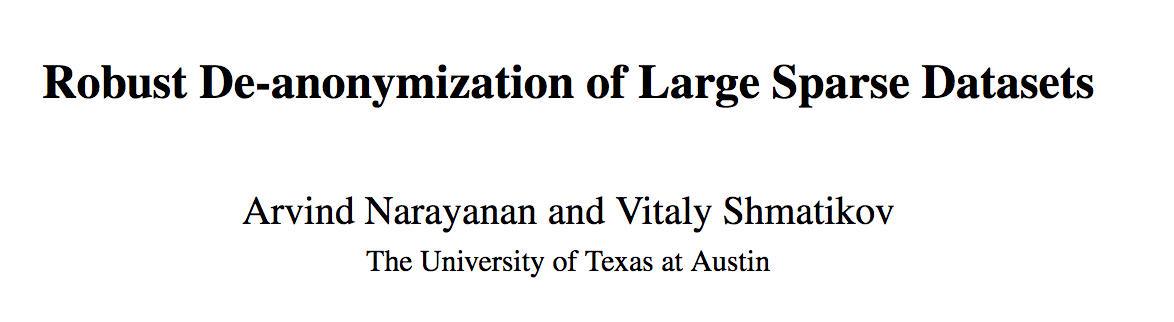
\includegraphics[width=0.9\textwidth]{figures/narayanan_robust_2008_title.png}
\end{center}
\vf

\tiny{\url{dx.doi.org/10.1109/SP.2008.33}}
\end{frame}
%%%%%%%%%%%%%%%%%%%%%%%%%%
\begin{frame}

\begin{center}

\includegraphics[width=0.9\textwidth]{figures/singal_netflix_2009_title.png}
\end{center}


\begin{quote}
``[M]ovie and rating data contains information of a more highly personal and sensitive nature [sic]. The member's movie data exposes a Netflix member's personal interest and/or struggles with various highly personal issues, including sexuality, mental illness, recovery from alcoholism, and victimization from incest, physical abuse, domestic violence, adultery, and rape.''  \href{http://www.wired.com/2009/12/netflix-privacy-lawsuit/}{(Singel, 2009)}
\end{quote}

\end{frame}
%%%%%%%%%%%%%%%%%%%%%%%%%%%
\begin{frame}

``Five safes'' data protection plan \href{http://rsss.anu.edu.au/sites/default/files/Ritchie_5safes.pdf}{(Desai et al 2016)}
\begin{itemize}
\item Safe projects
\pause
\item Safe people
\pause
\item Safe data
\pause
\item Safe settings
\pause
\item Safe output
\end{itemize}

\end{frame}
%%%%%%%%%%%%%%%%%%%%%%%%%%%
\begin{frame}

\begin{itemize}
\item With a strong data protection plan most computational social science is minimal risk
\pause
\item More ideas \href{https://www.bitbybitbook.com/en/1st-ed/ethics/dilemmas/info-risk/}{\textit{Bit by Bit}, Sec 6.6.2}
\end{itemize}

\end{frame}
%%%%%%%%%%%%%%%%%%%%%%%%%%%
\begin{frame}

\begin{center}
\Large{Privacy}
\end{center}

\end{frame}
%%%%%%%%%%%%%%%%%%%%%%%%%%%
\begin{frame}

What is privacy?

\end{frame}
%%%%%%%%%%%%%%%%%%%%%%%%%%%
\begin{frame}

Simple idea: Public/private dichotomy

\end{frame}
%%%%%%%%%%%%%%%%%%%%%%%%%%%
\begin{frame}

\begin{center}
\only<1>{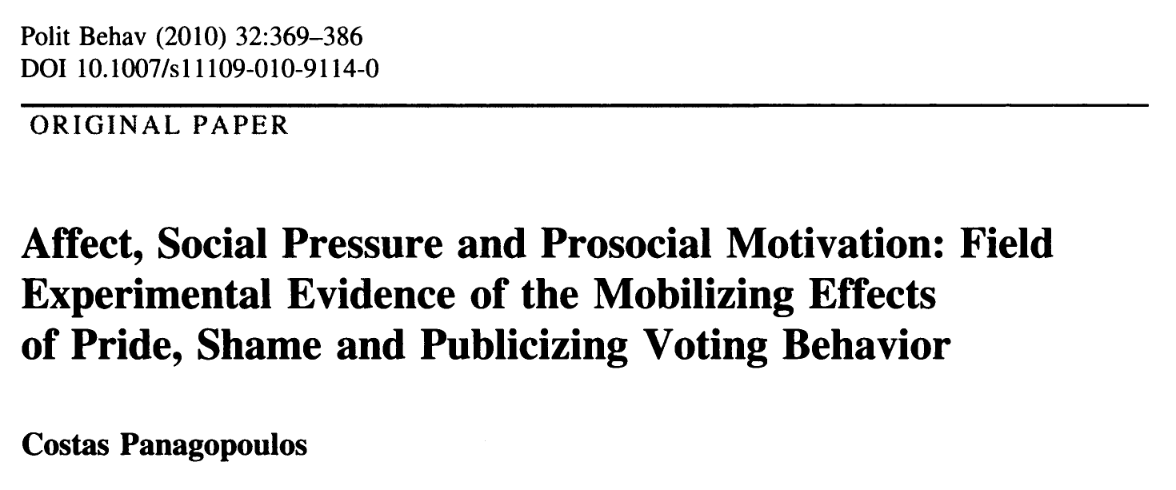
\includegraphics[width=0.9\textwidth]{figures/panagopoulos_affect_2010_title}}
\only<2>{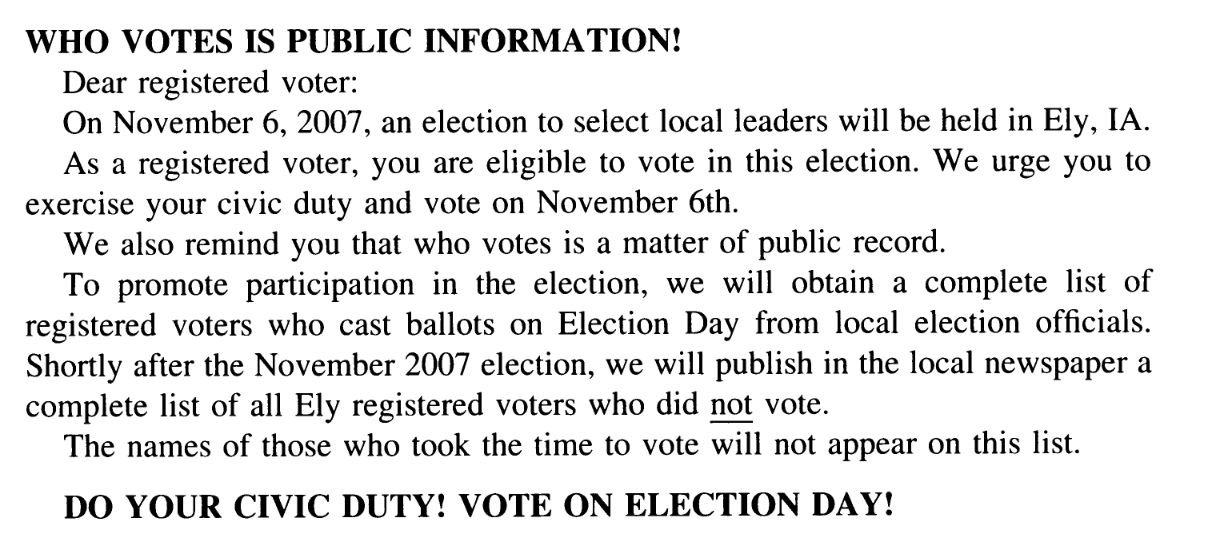
\includegraphics[width=0.9\textwidth]{figures/panagopoulos_affect_2010_iowa}}
\end{center}

\vf
\tiny{\url{http://www.jstor.org/stable/40960943}}

\end{frame}
%%%%%%%%%%%%%%%%%%%%%%%%%%%
\begin{frame}

\begin{itemize}
\item Simple idea: Public/private dichotomy
\item Better idea: contextual integrity (Nissenbaum), think about flows of information
\end{itemize}

\end{frame}
%%%%%%%%%%%%%%%%%%%%%%%%%%%
\begin{frame}

Key idea is ``context-relative informational norms''\\
\begin{itemize}
\item actors (subject, sender, recipient)
\item attributes (types of information)
\item transmission principles (constraints under which information flows)
\end{itemize}

\end{frame}
%%%%%%%%%%%%%%%%%%%%%%%%%%%
\begin{frame}

\begin{center}
\Large{Making decisions in the face of uncertainty}
\end{center}

\end{frame}
%%%%%%%%%%%%%%%%%%%%%%%%%%%
\begin{frame}

Simple idea: Better safe than sorry (``precautionary principle'')

\end{frame}
%%%%%%%%%%%%%%%%%%%%%%%%%%%
\begin{frame}

Imagine a study similar to Emotional Contagion\\
\begin{itemize}
\item Someone might be harmed by the experiment
\pause
\item Someone might be harmed if the experiment was not performed
\end{itemize}

\vf
There is no risk-free approach.

\end{frame}
%%%%%%%%%%%%%%%%%%%%%%%%%%%
\begin{frame}

\begin{itemize}
\item Simple idea: Better safe than sorry (``precautionary principle'')
\pause
\item Better idea: There is no risk free approach, and we should not take a narrow-field of view.
\end{itemize}

\vf
For fuller elaboration, see Sunstein (2005) \href{https://www.amazon.com/Laws-Fear-Precautionary-Principle-Lectures/dp/0521615127}{Laws of Fear: Beyond the Precautionary Principle}
\end{frame}
%%%%%%%%%%%%%%%%%%%%%%%%%%%
\begin{frame}

Ways forward:\\
\begin{itemize}
\pause
\item minimal risk standard
\pause
\item power analysis
\pause
\item ethical-response surveys
\pause
\item staged trials
\end{itemize}

For more details, see \href{https://www.bitbybitbook.com/en/1st-ed/ethics/dilemmas/uncertainty/}{\textit{Bit by Bit}, Sec 6.6.4}
\end{frame}
%%%%%%%%%%%%%%%%%%%%%%%%%%%
\begin{frame}

Four areas of difficulty:
\begin{enumerate}
\item informed consent
\item informational risk
\item privacy
\item making decisions in the face of uncertainty
\end{enumerate}

\end{frame}
%%%%%%%%%%%%%%%%%%%%%%%%%%%
\begin{frame}

Fifth area of difficulty (not in book): \pause unanticipated secondary uses

\end{frame}
%%%%%%%%%%%%%%%%%%%%%%%%%%%
\begin{frame}

\begin{center}
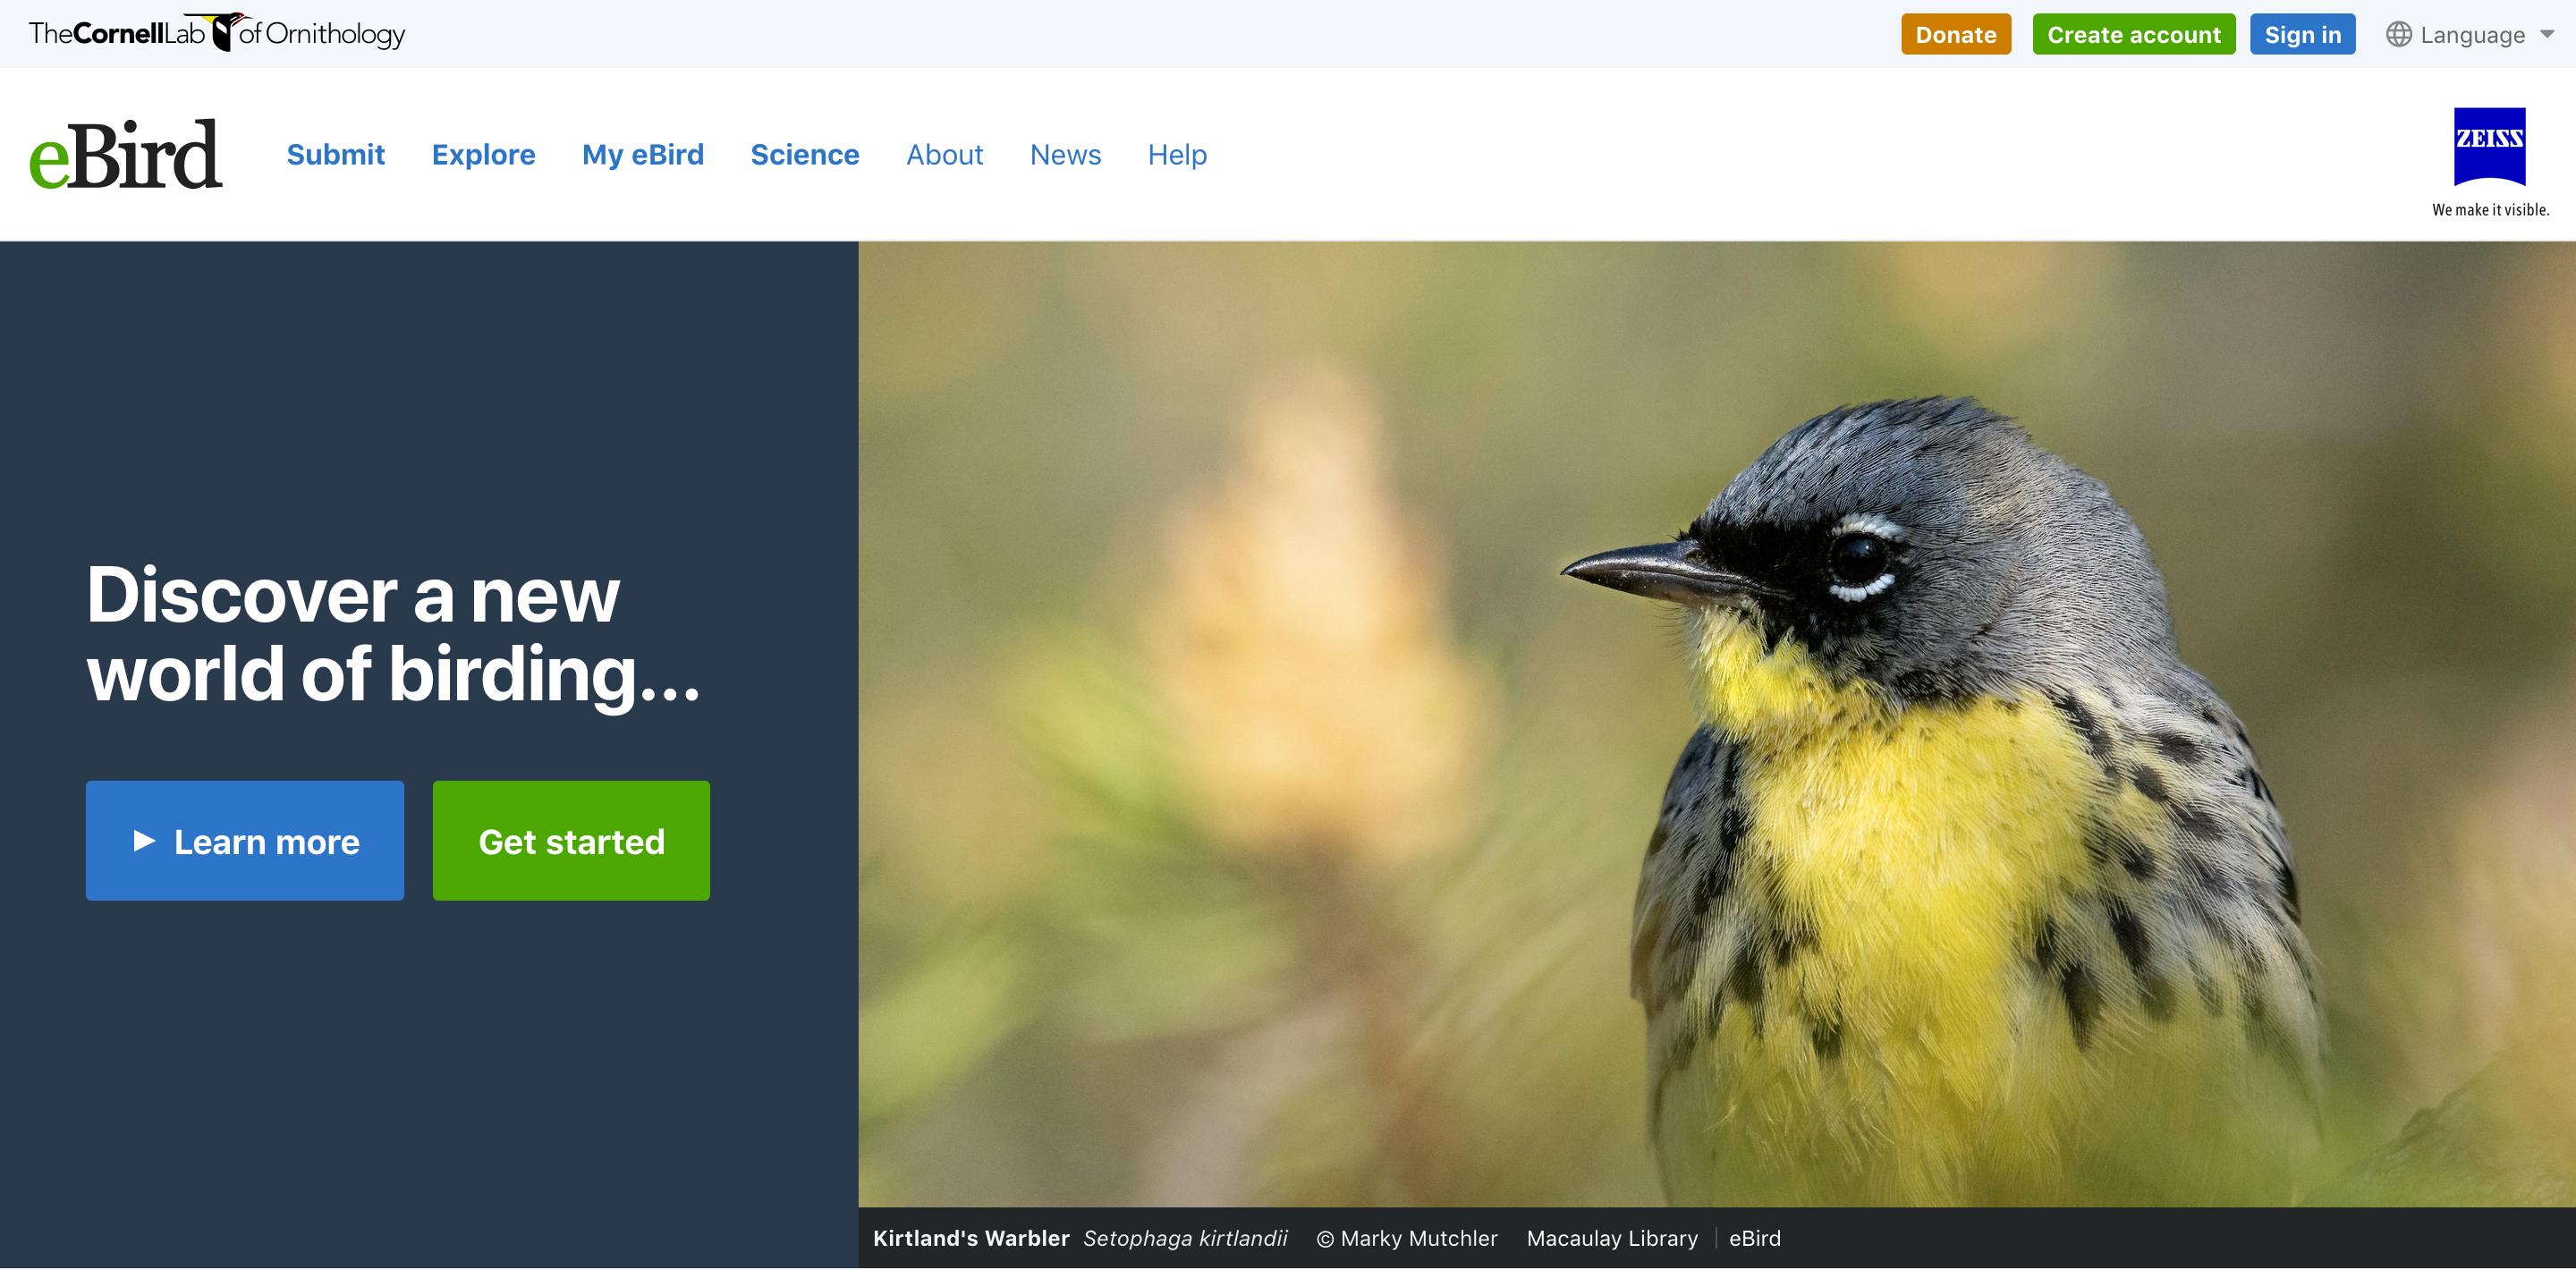
\includegraphics[width=\textwidth]{figures/ebird_screenshot}
\end{center}

\end{frame}
%%%%%%%%%%%%%%%%%%%%%%%%%%%
\begin{frame}

\begin{center}
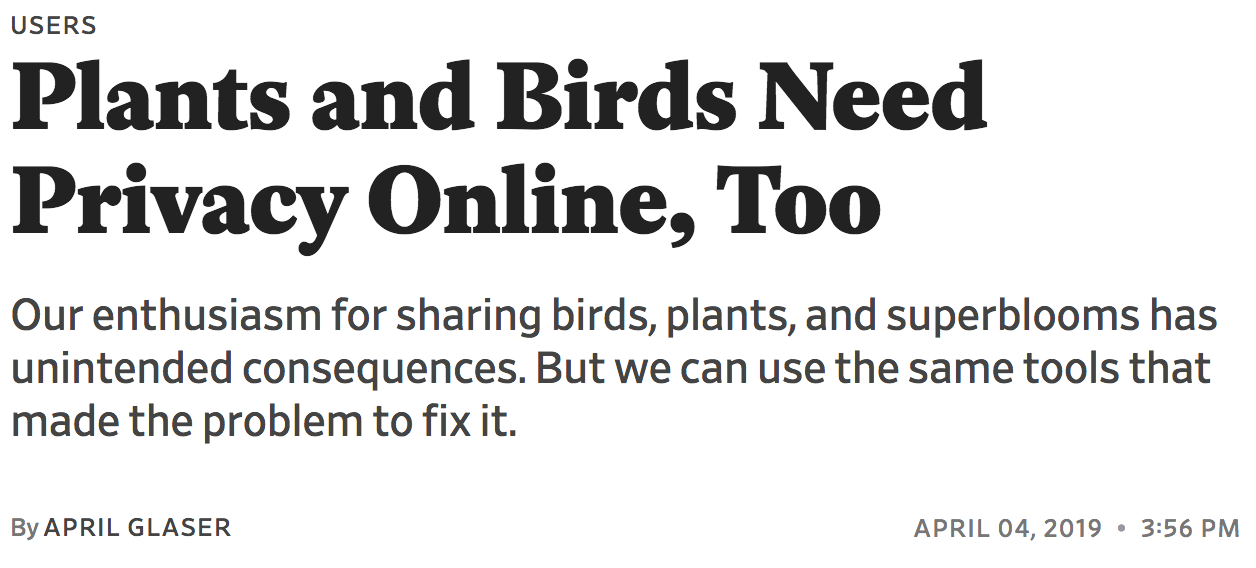
\includegraphics[width=0.8\textwidth]{figures/glaser_plants_2019_title}
\end{center}

\vfill
\url{https://slate.com/technology/2019/04/superbloom-california-nature-internet-collide-birds-poaching-science.html}
\end{frame}
%%%%%%%%%%%%%%%%%%%%%%%%%%%
\begin{frame}

\begin{center}
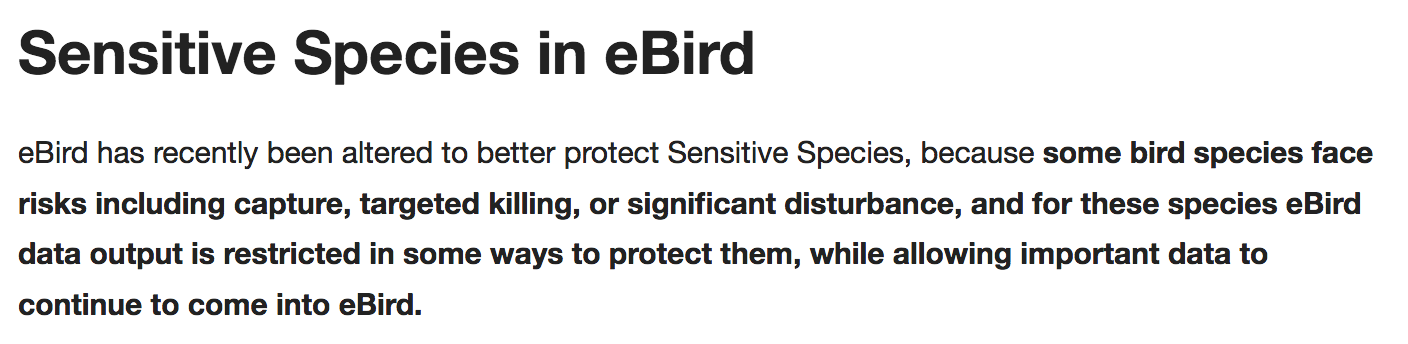
\includegraphics[width=\textwidth]{figures/ebird_sensitive_species}
\end{center}

\vfill
\url{https://help.ebird.org/customer/en/portal/articles/2885265-sensitive-species-in-ebird}
\end{frame}
%%%%%%%%%%%%%%%%%%%%%%%%%%
\begin{frame}

\begin{itemize}
\item Question: How would Lex Luther use this?
\item Requires adversarial thinking
\end{itemize}

\end{frame}
%%%%%%%%%%%%%%%%%%%%%%%%%%%
\begin{frame}

Practical advice:
\begin{itemize}
\item IRB is a floor not a ceiling
\pause
\item Put yourself in everyone else's shoes
\pause
\item Think of research ethics as continuous not discrete
\pause
\item Not in book: Think of ethics as a research opportunity
\end{itemize}

\end{frame}
%%%%%%%%%%%%%%%%%%%%%%%%%%%
\begin{frame}

\begin{center}
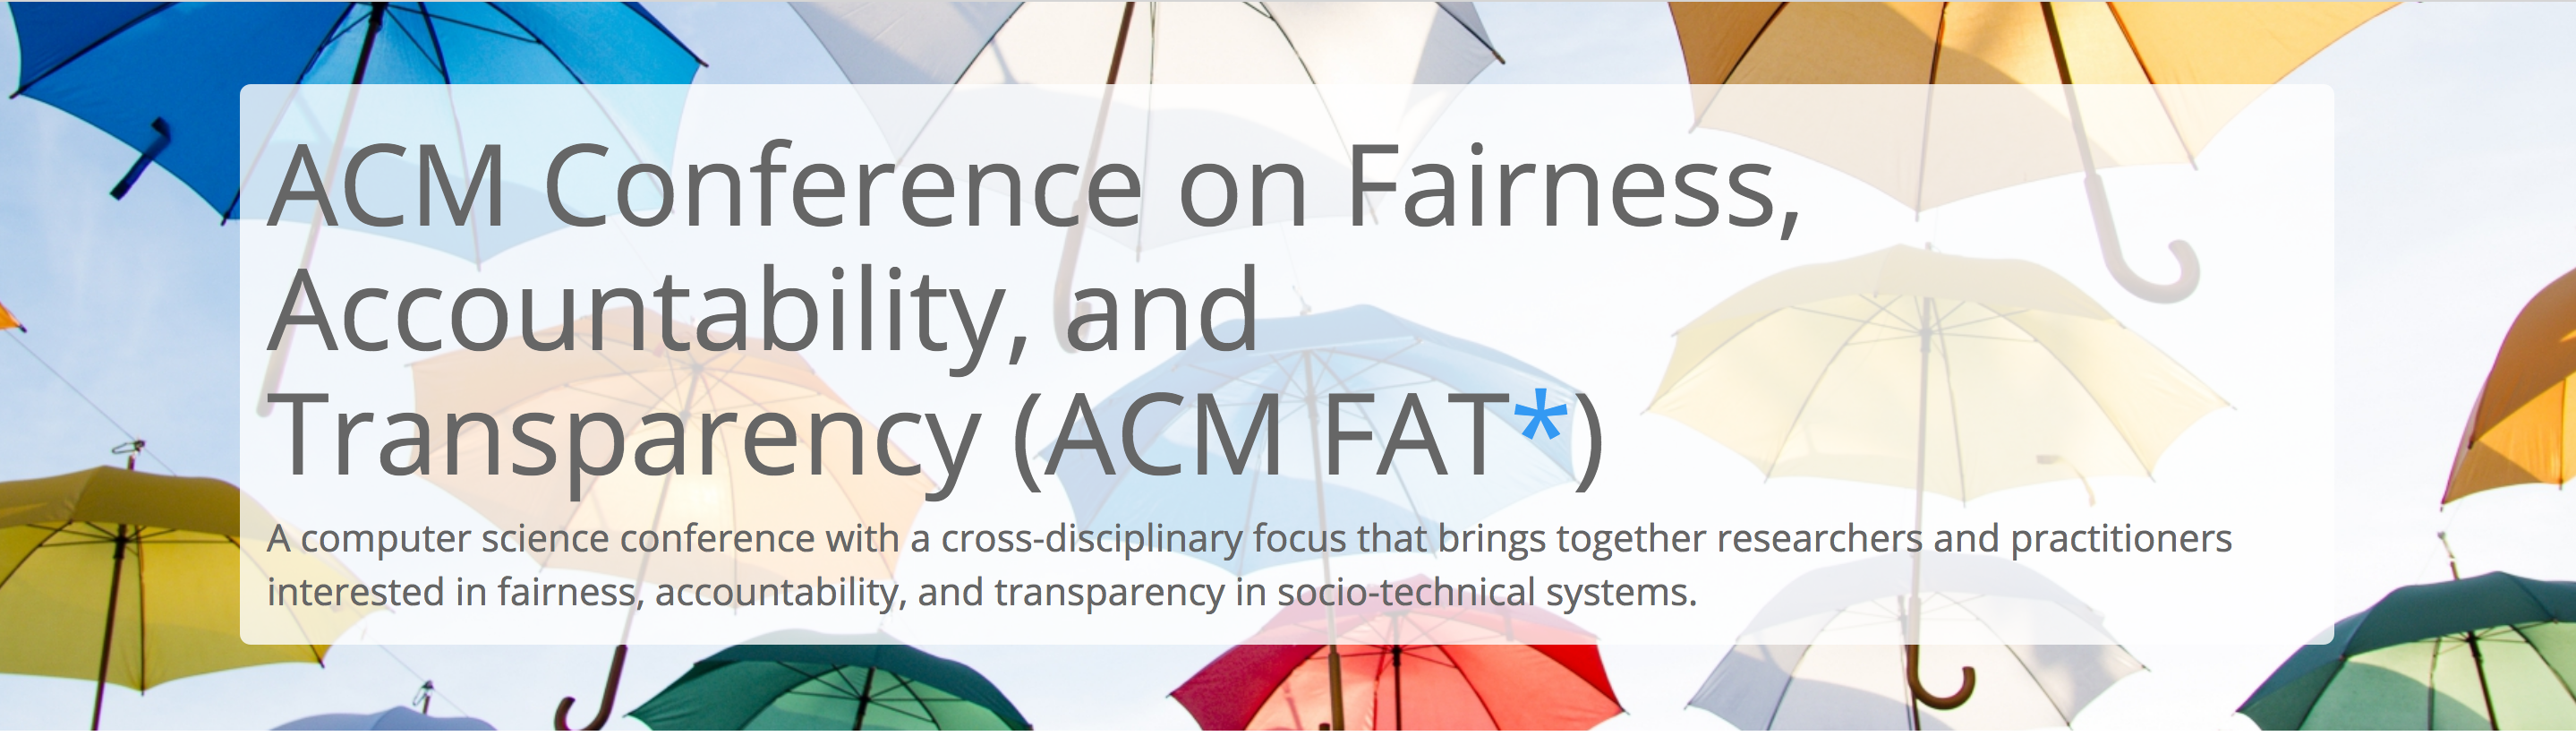
\includegraphics[width=\textwidth]{figures/fat_star}
\end{center}

\vf
\url{https://fatconference.org/}
\end{frame}
%%%%%%%%%%%%%%%%%%%%%%%%%%%
\begin{frame}

Next step: Your turn.\\
You will work in groups to analyze a real case and apply these ideas. 

\end{frame}
%%%%%%%%%%%%%%%%%%%%%%%%%%%
\begin{frame}

\begin{center}
\LARGE
Questions?
\end{center}

\end{frame}
%%%%%%%%%%%%%%%%%%%%%%%%%%%

\end{document}
